\documentclass[11pt,a4paper]{article}
\usepackage[utf8]{inputenc}
\usepackage[inner=2.5cm,outer=2.5cm, tmargin=2.5cm,bmargin=2.5cm]{geometry}
\usepackage{amsmath}
\usepackage{relsize,amsfonts}
\usepackage{enumitem}
\usepackage{graphicx}

\newcommand\bigexists{%
  \mathop{\lower0.75ex\hbox{\ensuremath{%
    \mathlarger{\mathlarger{\mathlarger{\mathlarger{\exists}}}}}}}%
  \limits}
  
\newcommand\bigforall{%
  \mathop{\lower0.75ex\hbox{\ensuremath{%
    \mathlarger{\mathlarger{\mathlarger{\mathlarger{\forall}}}}}}}%
  \limits}
  
\title{Wspomaganie Decyzji w Warunkach Ryzyka\\\large \medskip Projekt: WDWR 25406\\}
\author{Krzysztof Rudnicki 307585}
\date{\today}

\begin{document}

\maketitle

\section*{Treść zadania}
\addcontentsline{toc}{section}{Treść zadania}
Rozważmy następujące zagadnienie planowania produkcji:

\begin{itemize}
  \item Przedsiębiorstwo wytwarza 4 produkty P1,...,P4 na następujących maszynach: 4 szlifierkach, 
  2 wiertarkach pionowych, 3 wiertarkach poziomych, 1 frezarce i 1 tokarce. Wymagane czasy produkcji 
  1 sztuki produktu (w godzinach) w danym procesie obróbki zostały przedstawione w poniższej tabeli:\\
  \begin{center}
  \begin{tabular}{l*{4}{c}}
  	\hline
              			& P1 & P2 & P3 & P4 \\
	\hline
	Szlifowanie 		& 0,4 & 0,6 & - & - \\
	Wiercenie pionowe   & 0,2 & 0,1 & - & 0,6 \\
	Wiercenie poziome 	& 0,1 & - & 0,7 & -  \\
	Frezowanie  	 	& 0,06 & 0,04 & - & 0,05 \\
	Toczenie	     	& - & 0,05 & 0,02 & - \\
	\hline
	\end{tabular}
	\end{center}

  \item Dochody ze sprzedaży produktów (w zł/sztukę) określają składowe wektora 
  $\mathbf{R} = (R_{1},...,R_{4})^{T}$. Wektor $\mathbf{R}$ opisuje 4-wymiarowy rozkład 
  \textit{t}-Studenta z 4 stopniami swobody, którego wartości składowych zostały zawężone do 
  przedziału $[5;12]$. Wektor wartości oczekiwanych $\mu$ oraz macierz kowariancji 
  $\Sigma$ niezawężonego rozkładu \textit{t}-Studenta są następujące:
  \begin{displaymath}
\mathbf{\mu} = 
 \begin{pmatrix}
  9 \\ 8 \\ 7 \\ 6 \\  
 \end{pmatrix},
 \mathbf{\Sigma} = 
 \begin{pmatrix}
  16 & -2 & -1 & -3 \\
  -2 & 9 & -4 & -1 \\ 
  -1 & -4 & 4 & 1 \\
  -3 & -1 & 1 & 1 \\  
 \end{pmatrix}
  \end{displaymath}
  
  \item Istnieją ograniczenia rynkowe na liczbę sprzedawanych produktów w danym miesiącu:
  \begin{center}
  \begin{tabular}{l*{4}{c}}
  	\hline
              			& P1 & P2 & P3 & P4 \\
	\hline
	Styczeń 			& 200 & 0 & 100 & 200 \\
	Luty   				& 300 & 100 & 200 & 200 \\
	Marzec 				& 0 & 300 & 100 & 200  \\
	\hline
	\end{tabular}
	\end{center}
	
	\item Jeżeli sprzedaż danego produktu przekracza 80 procent ilości jaką może wchłonąć rynek, 
    jego dochód spada o 20 procent.
	
	\item Istnieje możliwość składowania do 200 sztuk każdego produktu w danym czasie w cenie 1 zł/sztukę 
    za miesiąc. W chwili obecnej (grudzień) w magazynach znajduje się po 50 sztuk każdego produkt. 
    Istnieje wymaganie, aby tyle pozostało również pod koniec marca.
	
	\item Przedsiębiorstwo pracuje 6 dni w tygodniu w systemie dwóch zmian. Każda zmiana trwa 8 godzin. 
    Można założyć, że każdy miesiąc składa się z 24 dni roboczych.
\end{itemize}

\section*{Polecenia}
\addcontentsline{toc}{section}{Polecenia}
\begin{enumerate}
  \item Zaproponować jednokryterialny model wyboru w warunkach ryzyka z wartością oczekiwaną jako 
  miarą zysku. Wyznaczyć rozwiązanie optymalne.
  \item Jako rozszerzenie powyższego zaproponować dwukryterialny model zysku i ryzyka ze średnią 
  jako miarą zysku i średnią różnicą Giniego jako miarą ryzyka. Dla decyzji 
  $\mathbf{x}\in Q$ średnia różnica Giniego jest definiowana jako 
  $\Gamma(\mathbf{x})=\frac{1}{2}\sum_{t'=1}^{T}\sum_{t"=1}^{T}\lvert r_{t'}(\mathbf{x})-r_{t"}(\mathbf{x})\rvert p_{t'}p_{t"}$, gdzie $r_{t'}(\mathbf{x})$ 
  oznacza realizację dla scenariusza t, $p_{t}$ prawdopodobieństwo scenariusza t.
  \begin{enumerate}
    \item Wyznaczyć obraz zbioru rozwiązań efektywnych w przestrzeni zysk-ryzyko.
    \item Wskazać rozwiązania efektywne minimalnego ryzyka i maksymalnego zysku. Jakie odpowiadają im 
    wartości w przestrzeni ryzyko-zysk?
    \item Wybrać trzy dowolne rozwiązania efektywne. Sprawdzić, czy zachodzi pomiędzy nimi relacja 
    dominacji stochastycznej pierwszego rzędu. Wyniki skomentować, odnieść do ogólnego przypadku.
  \end{enumerate}
\end{enumerate}

\section{Jednokryterialny model wyboru}
Model jednokryterialny wyboru w warunkach ryzyka został zaprojektowany w celu identyfikacji rozwiązania 
optymalnego poprzez maksymalizację oczekiwanej wartości zysku. Wartość oczekiwana jest kalkulowana na 
podstawie scenariuszy generowanych zgodnie z rozkładem \textit{t}-Studenta wykorzystującym parametry 
określone w zadaniu. W analizie założono równomierne prawdopodobieństwo występowania wszystkich 
scenariuszy.
\subsection{Parametry modelu}
Wszystkie parametry modelu zostały przedstawione w tabeli poniżej wraz z ich szczegółowymi opisami. 
Identyczne nazewnictwo zostało zastosowane w implementacji modelu. Dla parametrów będących wektorami 
i macierzami, w nawiasach kwadratowych określono ich wymiary, odnosząc się do odpowiednich parametrów liczbowych.
\begin{table}[ht!]
\caption{Tabela zawierająca parametry modelu jednokryterialnego}
\label{tab:param}
\begin{tabular}{lp{9cm}}
    \hline
    Nazwa parametru      & Szczegółowy opis znaczenia \\
    \hline
    numberOfMachineTypes & Ilość typów maszyn (procesów) dostępnych w fabryce \\
numberOfMonths & Ilość miesięcy uwzględnionych w symulacji  \\
numberOfProductsTypes & Ilość typów produktów \\
numberOfScenarios & Ilość scenariuszy wygenerowanych do symulacji \\
machines[numberOfMachineTypes] & Wektor typów maszyn (procesów)\\
months[numberOfMonths] & Wektor miesięcy symulacji\\
products[numberOfProductsTypes] & Wektor typów produktów\\
machineCount[numberOfMachineTypes] & Wektor ilości maszyn danego typu\\
timeToProduce[numberOfMachineTypes][numberOfProductsTypes] & macierz czasów produkcji danego produktu na danej maszynie \\
maxProductsInMonth[numberOfMonths][numberOfProductsTypes] & macierz maksymalnej ilości produktów, jakie można sprzedać w danym miesiącu\\
numberOfHoursInFactory & Ilość godzin pracy fabryki w miesiącu\\
mu[numberOfProductsTypes] & Wektor wartości oczekiwanych rozkładu t-Studenta do generacji scenariuszy\\
sigma [numberOfProductsTypes][numberOfProductsTypes] & Macierz kowariancji dla rozkłady t-Studenta\\ 
sellProfit[numberOfScenarios][numberOfProductsTypes] & Macierz wygenerowanych sceniariuszy dochodów ze sprzedaży produktów\\
storageCost & Koszt trzymania jednej sztuki produktu w magazynie przez miesiąc \\
storageMax[numberOfProductsTypes] & Wektor maksymalnej pojemności magazynu dla każdego typu produktu \\
storageStart[numberOfProductsTypes] & Wektor ilości początkowej produktów w magazynie \\
    \hline
\end{tabular}
\end{table}

\subsection{Zmienne decyzyjne}
Zmienne decyzyjne stanowią wartości kontrolowane przez podmiot podejmujący decyzje i są fundamentalne dla rozwiązywanego problemu. Zadaniem optymalizatora jest wyznaczenie takich wartości tych zmiennych, które umożliwią osiągnięcie optymalnego rozwiązania. W tabeli zawierającej zmienne decyzyjne modelu zaprezentowano zmienne decyzyjne zastosowane w modelu wraz z ich szczegółowymi opisami. Przyjęto tę samą konwencję nazewnictwa, co w przypadku parametrów modelu.

\begin{table}[ht!]
\caption{Tabela zawierająca zmienne decyzyjne modelu}
\label{tab:var}
\begin{tabular}{lp{7.5cm}}
	\hline
    Nazwa zmiennej      & Szczegółowy opis znaczenia \\
        \hline
        produce[numberOfMonths][numberOfProductsTypes] & Macierz zawierające ilości wytwarzanych sztuk danego typu produktu w danym miesiącu \\
        sell[numberOfMonths][numberOfProductsTypes] & Macierz zawierająca ilości sprzedawanych sztuk danego typu produktu w danym miesiącu \\
        stock[numberOfMonths][numberOfProductsTypes] & Macierz zawierająca ilości sztuk danego typu produktu znajdujących się w magazynie w danym miesiącu \\
        workTime[numberOfMonths][numberOfMachineTypes][numberOfProductsTypes] & Macierz zawierająca czas pracy każdej maszyny dla każdego typu produktu w kazdym miesiącu \\
        if80prec[numberOfMonths][numberOfProductsTypes] & Macierz zmiennych binarnych (1 jeśli sprzedaż danego produktu w danym miesiącu przekroczyła 80\% wartości maksymalnej, 0 - w przeciwnym wypadku)\\
        lowerProfit[numberOfScenarios][numberOfMonths][numberOfProductsTypes] & Macierz przechowująca kwoty, jaką należy odjąć od zysków z poszczególnych typów produktów w poszczególnych miesiącach, ze względu na przekroczenie 80\% pojemności rynku. Zmienna niezbędna do wyeliminowania obecności zmiennej binarnej w funkcji oceny\\
	\hline
\end{tabular}
\end{table}

\subsection{Ograniczenia}
\begin{itemize}
\item Ograniczenie dolne wartości zmiennych decyzyjnych – wartości nie mogą być mniejsze od zera:
	\begin{equation}
	\bigforall_{\substack{
			m \in months \\ 
			p \in products \\
			mc \in machines}} workTime[m][mc][p] >=0
	\end{equation}
	\begin{equation}
	\bigforall_{\substack{
			m \in months \\ 
			p \in products}} produce[m][p] >=0
	\end{equation}
	\begin{equation}
	\bigforall_{\substack{
			m \in months \\ 
			p \in products}} sell[m][p] >=0
	\end{equation}
	\begin{equation}
	\bigforall_{\substack{
			m \in months \\ 
			p \in products}} stock[m][p] >=0
	\end{equation}
	\begin{equation}
	\bigforall_{\substack{
			i \in scenarios \\
			m \in months \\ 
			p \in products}} lowerProfit[i][m][p] >=0
	\end{equation}

\item Ograniczenie czasowe pracy maszyn - Każda maszyna może pracować maksymalnie \textit{numberOfHoursInFactory} godzin w miesiącu, zatem łączny czas pracy wszystkich maszyn danego typu nie może przekroczyć iloczynu liczby dostępnych maszyn tego typu i czasu \textit{numberOfHoursInFactory}.
	\begin{equation}
		\bigforall_{\substack{
			m \in months\\ 
			mc \in machines}}  \sum_{p \in products}
		(workTime[m][mc][p] <= machineCount[mc]*numberOfHoursInFactory)
	\end{equation}
    \item Ograniczenie wiążące czas pracy maszyn z produkcją - czas wykorzystania określonego typu maszyny jest równy sumie iloczynów liczby wytworzonych jednostek każdego produktu i czasu potrzebnego na obróbkę jednej jednostki tego produktu na danej maszynie:
	\begin{equation}
		\bigforall_{\substack{
			m \in months\\ 
			mc \in machines\\
			p \in products}} workTime[m][mc][p] == produce[m][p]*timeToProduce[mc][p]
	\end{equation}
    \item Ograniczenie maksymalnej sprzedaży wynikające z pojemności rynku w danym miesiącu:
	\begin{equation}
		\bigforall_{\substack{
			m \in months\\ 
			p \in products}} sell[m][p] == maxProductsInMonth[m][p]
	\end{equation}
	
    \item Warunki definiujące zmienną binarną przy przekroczeniu 80 procent chłonności rynku:
	\begin{equation}
		\bigforall_{\substack{
			m \in months\\ 
			p \in products}}  sell[m][p] <= 0.8*maxProductsInMonth[m][p] + 1000000 * if80prec[m][p]
	\end{equation}
	\begin{equation}
		\bigforall_{\substack{
			m \in months\\ 
			p \in products}} sell[m][p] >= 0.8*maxProductsInMonth[m][p] * if80prec[m][p]
	\end{equation}
	
    \item Ograniczenia linearyzujące oddziaływanie zmiennych binarnych na funkcję celu:
	\begin{equation}
		\bigforall_{\substack{
			i \in scenarios\\			
			m \in months\\ 
			p \in products}} lowerProfit[i][m][p] <= 1000000 * if80prec[m][p]
	\end{equation}
	\begin{equation}
		\bigforall_{\substack{
			i \in scenarios\\			
			m \in months\\ 
			p \in products}} lowerProfit[i][m][p] <= 0.2 * sell[m][p]*sellProfit[i][p]
	\end{equation}
	\begin{multline}
		\bigforall_{\substack{
			i \in scenarios\\			
			m \in months\\ 
			p \in products}} 0.2 * sell[m][p]*sellProfit[i][p] - lowerProfit[i][m][p] +\\ 1000000 * if80prec[m][p] <= 1000000;
	\end{multline}
	
    \item Ograniczenie sprzedaży do liczby sztuk wyprodukowanych oraz dostępnych w magazynie. Dla pierwszego miesiąca ograniczenie przyjmuje formę:
	\begin{equation}
		\bigforall_{\substack{
			m \in months\\ 
			p \in products}} sell[m][p] <= produce[m][p]+storageStart[p]
	\end{equation}
	Dla każdego następnego miesiąca:
	\begin{equation}
		\bigforall_{\substack{
			m \in months\\ 
			p \in products}} sell[m][p] <= produce[m][p] + stock[m-1][p]
	\end{equation}
	
    \item Ograniczenie określające stan magazynu na koniec miesiąca jako różnicę między sumą produktów wyprodukowanych i dostępnych na początku miesiąca a liczbą sprzedanych jednostek. Dla pierwszego miesiąca:
	\begin{equation}
		\bigforall_{\substack{
			m \in months\\ 
			p \in products}} stock[m][p]==(produce[m][p] + storageStart[p])-sell[m][p]
	\end{equation}
	Dla każdego następnego miesiąca:
	\begin{equation}
		\bigforall_{\substack{
			m \in months\\ 
			p \in products}} stock[m][p]==(produce[m][p] + stock[m-1][p])-sell[m][p]
	\end{equation}

\end{itemize}
\subsection{Funkcja celu}
Funkcja celu w modelu jednokryterialnym polega na maksymalizacji wartości oczekiwanej zysku ze wszystkich analizowanych scenariuszy. W każdym ze scenariuszy zastosowano funkcję zysku o następującej postaci
\begin{multline}
\bigforall_{\substack{
			i<nScernarios\\ 
			i \in N}}  
	profit[i] =\sum_{m \in months} \sum_{p \in products}
		(sell[m][p]\cdot sellProfit[i][p] \\ -lowerProfit[i][m][p]-stock[m][p]*storageCost)
\end{multline}
 


\subsection{Implementacja modelu}
\subsubsection{Generacja scenariusz dochodów ze sprzedaży}
Przychody ze sprzedaży poszczególnych typów produktów definiowane są przez wektor losowy opisany w treści zadania. W celu wygenerowania wektorów reprezentujących poszczególne scenariusze przychodów zastosowano bibliotekę MASS języka R. Implementacja została wykonana w środowisku R Studio IDE, a skrypt generujący dane zapisano w pliku dołączonym jako załącznik 1 - \textit{t-student.R}. W ramach przeprowadzonej symulacji wygenerowano 1000 scenariuszy realizacji przychodów.

\subsubsection{Model}
Model zaimplementowano w środowisku IBM ILOG CPLEX Optimization Studio z wykorzystaniem solvera CPLEX. Nazewnictwo parametrów oraz zmiennych decyzyjnych jest zgodne z opisem zawartym w tabelach \ref{tab:param} i \ref{tab:var}. Plik \textit{wdwr17421-1.dat} (załącznik 2) zawiera definicje parametrów modelu, natomiast plik \textit{wdwr17421-1.mod} (załącznik 3) obejmuje wczytywanie parametrów, definicje zmiennych decyzyjnych, funkcji celu oraz ograniczeń modelu. W celu uproszczenia implementacji przyjęto numeryczne oznaczenia dla miesięcy, produktów oraz procesów technologicznych. Miesiące numerowane są chronologicznie, produkty zgodnie z indeksem występującym w nazwie (P1-P4), natomiast procesy technologiczne według poniższej sekwencji:
\begin{enumerate}
\item Szlifowanie,
\item Wiercenie pionowe,
\item Wiercenie poziome,
\item Frezowanie,
\item Toczenie.
\end{enumerate}

\subsection{Rozwiązanie}
Rozwiązanie optymalne modelu maksymalizacji wartości oczekiwanej zysku zostało wyznaczone przy użyciu solvera CPLEX. 
Maksymalna wartość oczekiwana zysku wynosi około 11036,12 zł. 
Optymalne wartości zmiennych decyzyjnych przedstawiają się następująco:
\begin{displaymath}
\mathbf{sell} = 
 \begin{pmatrix}
  160 & 0 & 80 & 160 \\
  240 & 80 & 160 & 160 \\ 
  0 & 240 & 80 & 160 \\  
 \end{pmatrix},
 \mathbf{if80prec} = 
 \begin{pmatrix}
  0 & 1 & 0 & 0 \\
  0 & 0 & 0 & 0 \\ 
  1 & 0 & 0 & 0 \\  
 \end{pmatrix},
\end{displaymath}
\begin{displaymath}
\mathbf{stock} = 
 \begin{pmatrix}
  0 & 50 & 0 & 0 \\
  0 & 0 & 0 & 0 \\ 
  50 & 50 & 50 & 50 \\  
 \end{pmatrix},
 \mathbf{produce} = 
 \begin{pmatrix}
  110 & 0 & 30 & 110 \\
  240 & 30 & 160 & 160 \\ 
  50 & 290 & 130 & 210 \\  
 \end{pmatrix} 
\end{displaymath}

Czasem pracy poszczególnych typów maszyn dla różnych typów produktów w każdym miesiącu obrazują następujące macierze:
\begin{displaymath}
 \mathbf{workTime[1]} =
 \begin{pmatrix}
	44 & 0 & 0 & 0 \\
	22 & 0 & 0 & 66 \\ 
	11 & 0 & 35 & 0 \\
	6.6 & 0 & 0 & 5.5 \\
	0 & 0 & 1 & 0 \\  
 \end{pmatrix},
 \mathbf{workTime[2]} =
 \begin{pmatrix}
	96 & 18 & 0 & 0 \\
	48 & 3 & 0 & 96 \\ 
	24 & 0 & 140 & 0 \\
	14.4 & 1.2 & 0 & 8 \\ 
	0 & 1.5 & 4 & 0 \\
 \end{pmatrix},
\end{displaymath}
\begin{displaymath}
 \mathbf{workTime[3]} =
 \begin{pmatrix}
	20 & 174 & 0 & 0 \\
	10 & 29 & 0 & 126 \\ 
	5 & 0 & 105 & 0 \\
	3 & 11.6 & 0 & 10.5 \\ 
	0 & 14.5 & 3 & 0 \\
 \end{pmatrix}
\end{displaymath}

Ze względu na znaczne rozmiary macierzy lowerProfit pominięto jej przedstawienie w niniejszym raporcie. Kompletne wyniki działania solvera zostały załączone do dokumentu jako załącznik 4.
\subsection{Wnioski}
Na podstawie przeprowadzonej analizy można stwierdzić, że zdolności produkcyjne przedsiębiorstwa znacznie przewyższają chłonność rynku. W kontekście maksymalizacji zysku, w określonych miesiącach ekonomicznie uzasadniona jest sprzedaż poszczególnych produktów mimo przekroczenia 80\% pojemności rynkowej. Optymalna strategia nie wymaga gromadzenia zapasów ponad obligatoryjne minimum magazynowe.

\section{Model dwukryterialny zysku i ryzyka}
\subsection{Model zadania}
Model przedsiębiorstwa został zachowany w niezmienionej formie w porównaniu do pierwszej części zadania. Miarą zysku pozostaje wartość oczekiwana, która w przypadku scenariuszy o równym prawdopodobieństwie odpowiada wartości średniej. Miara ryzyka w niniejszym zadaniu jest reprezentowana przez średnią różnicę Giniego określoną następującym wzorem:
\begin{equation}
\Gamma(\mathbf{x})=\frac{1}{2}\sum_{t'=1}^{T}\sum_{t"=1}^{T}\lvert r_{t'}(\mathbf{x})-r_{t"}(\mathbf{x})\rvert p_{t'}p_{t"}, 
\end{equation}
gdzie $r_{t'}(\mathbf{x})$ oznacza realizację zysku dla scenariusza $t'$, a $p_{t}$ - prawdopodobieństwo wystąpienia scenariusza $t$.

W kontekście przyjętych w projekcie oznaczeń, wyrażenie definiujące miarę ryzyka przyjmuje następującą postać:
\begin{equation}
riskMeasureGini = \frac{1}{2}\cdot\sum_{t1 \in scenarios}\sum_{t2 \in scenarios} \lvert profit[t1]-profit[t2] \rvert \cdot \frac{1}{numberOfScenarios} \cdot \frac{1}{numberOfScenarios} 
\end{equation}

\subsection{Model preferencji}
Model preferencji oparto na minimalizacji ryzyka przy zadanym poziomie średniego zysku.
\begin{equation}
averageProfit<minimalAverageProfit
\end{equation}
\begin{equation}
minimize riskMeasureGini
\end{equation}
minimalAverageProfit stanowi dodatkowy parametr modelu. Załączniki 5 i 6 zawierają pliki z parametrami i modelem zadania dwukryterialnego wyboru - pliki źródłowe przeznaczone dla solvera CPLEX. 

\subsection{Zbiór rozwiązań efektywnych w przestrzeni ryzyko-zysk}
Na rysunku \ref{fig:profit-risk} zaprezentowano rozwiązania efektywne modelu w przestrzeni ryzyko-zysk. Niebieskie trójkąty oznaczają rozwiązania efektywne dla różnych wartości wymaganego poziomu zysku. Uwzględniając ograniczenia obliczeniowe komputera, wygenerowano 52 równomiernie rozmieszczone rozwiązania, z których każde bazuje na 30 scenariuszach. Wprowadzono ograniczenie czasowe działania solvera dla pojedynczego rozwiązania na poziomie 5 minut. Całkowity czas obliczeń przekroczył 3 godziny. Załączniki 7 i 8 obejmują pliki parametrów oraz modelu wraz ze skryptem dla solvera CPLEX, które zostały wykorzystane do uzyskania rozwiązań. Kolorem żółtym wyróżniono rozwiązanie maksymalnego zysku oraz minimalnego ryzyka. Wartości odpowiadające tym rozwiązaniom przedstawiono w tabeli \ref{tab:min-max}.
\begin{figure}[ht!]
\centering
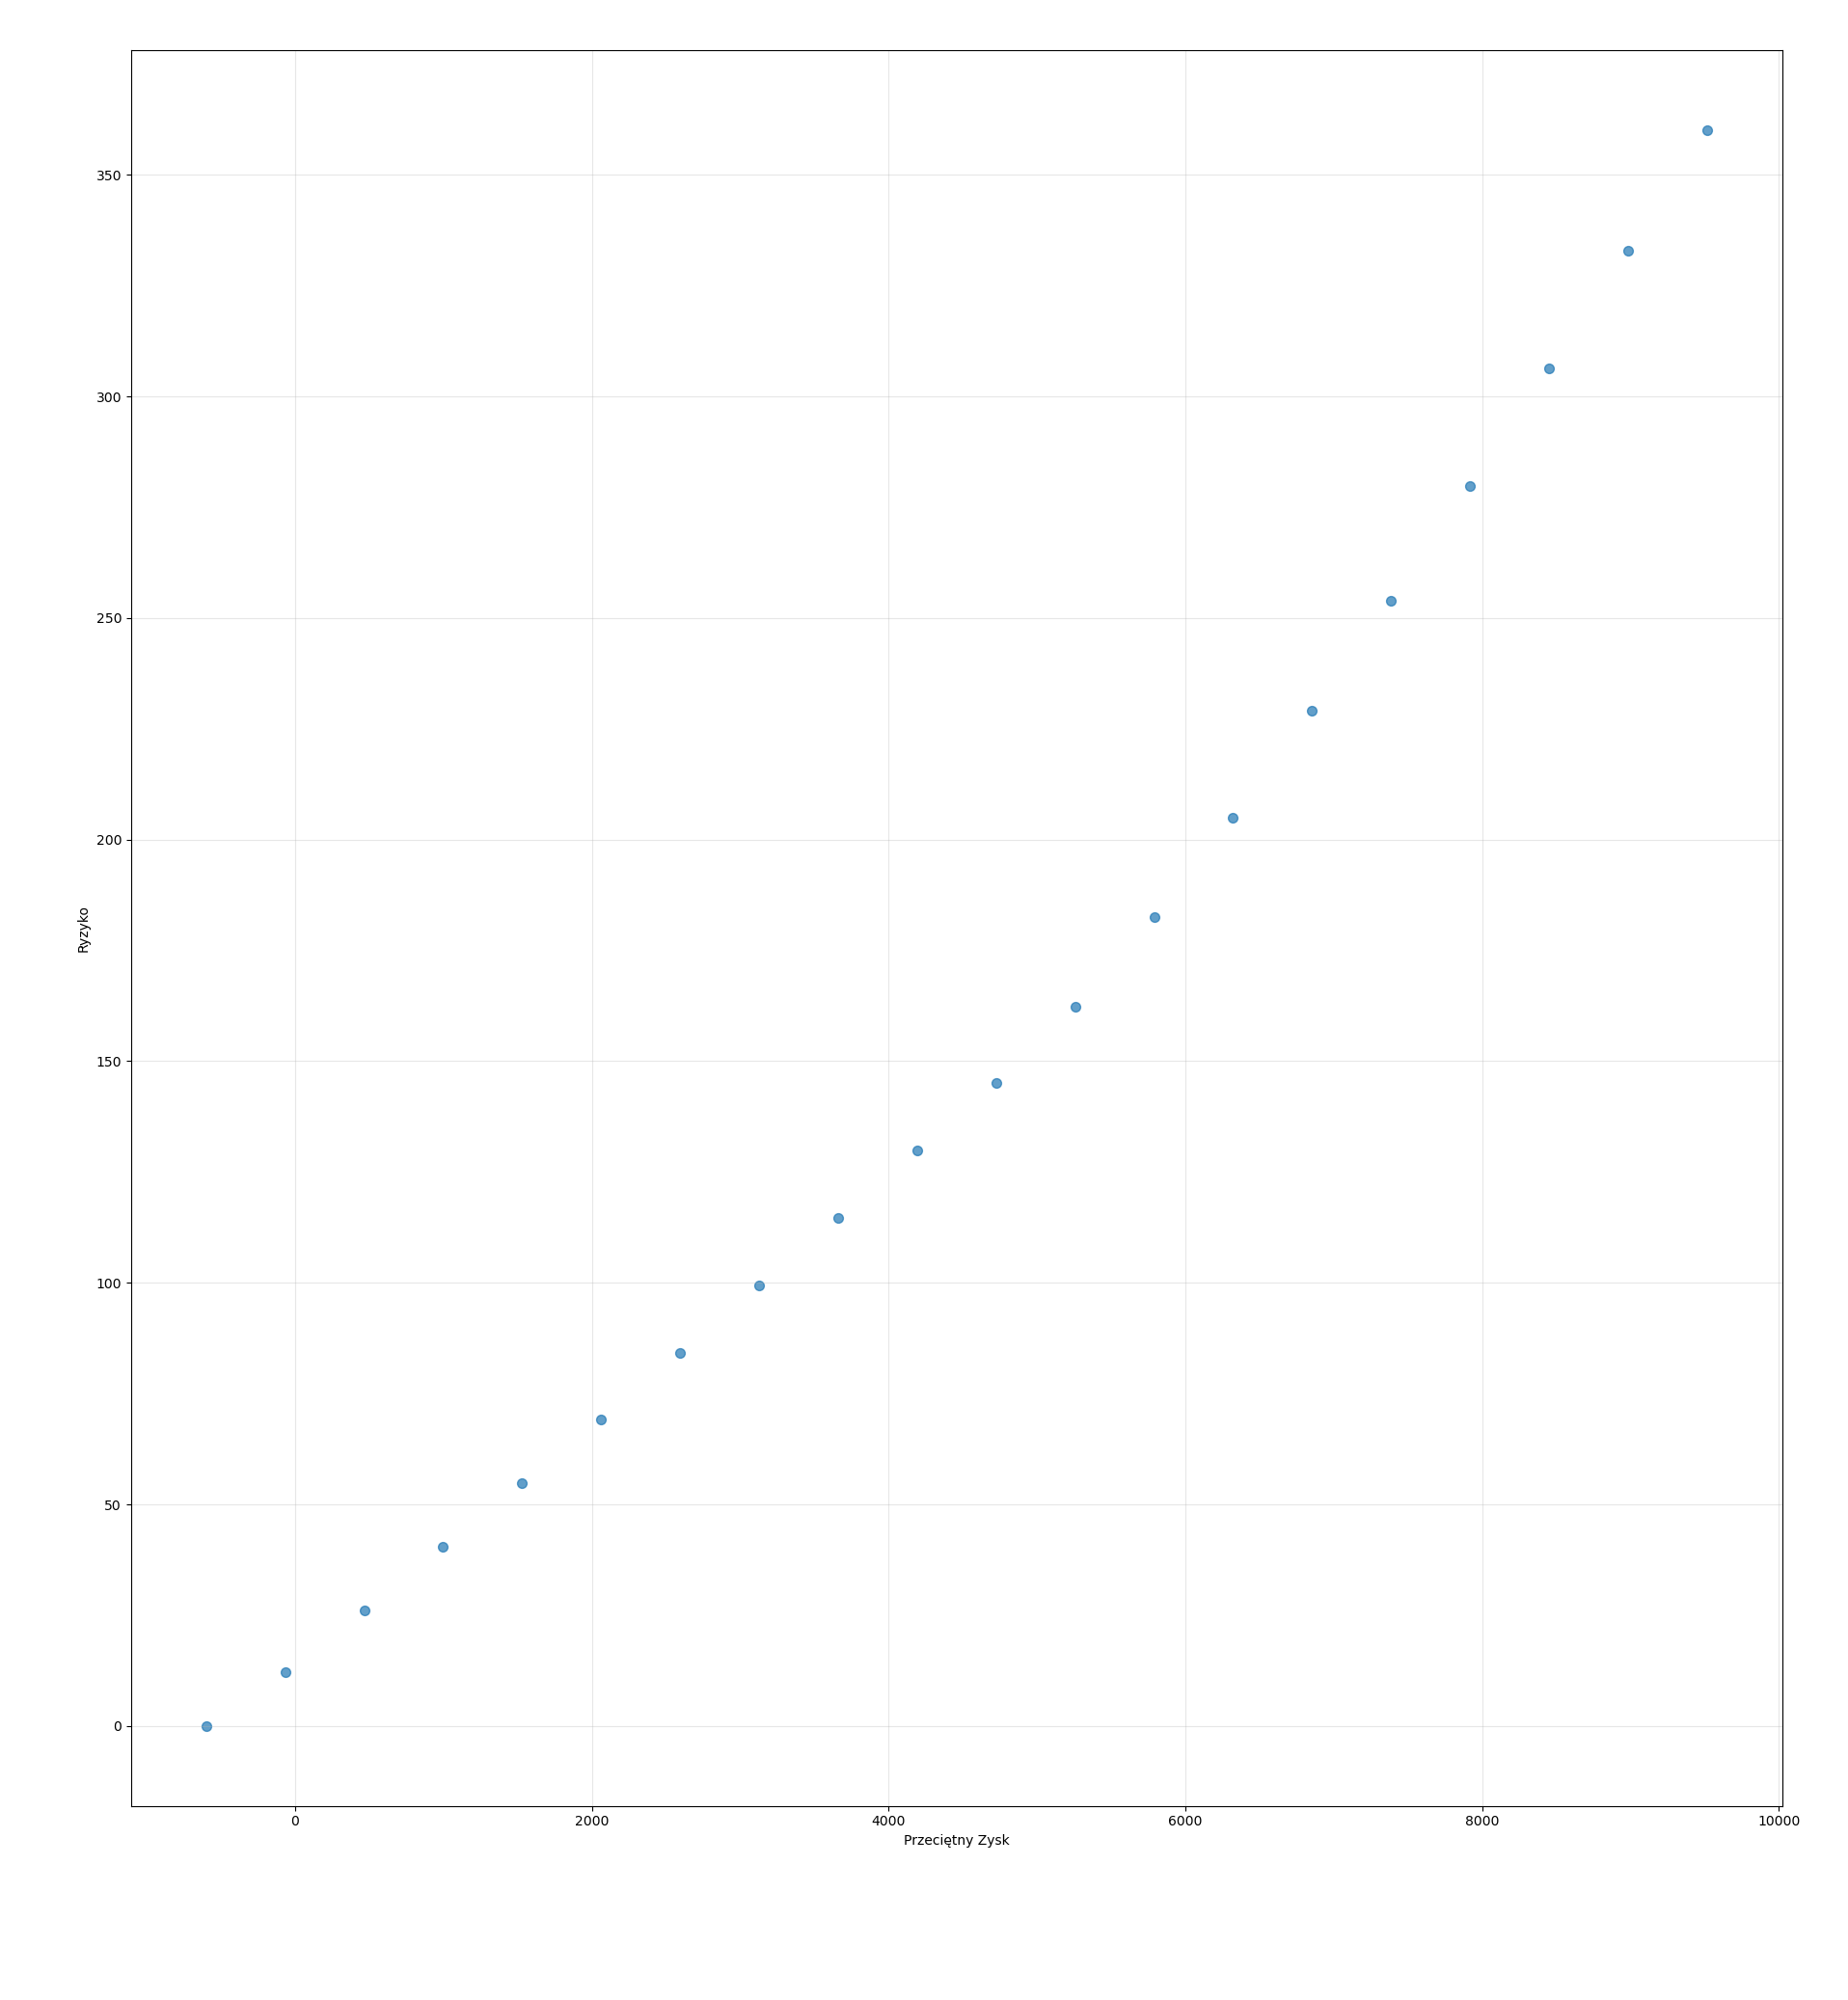
\includegraphics[width=0.8\textwidth]{graphics/ryzyko_zysk_wykres.png}
\caption{Obraz zbioru rozwiązań efektywnych w przestrzeni ryzyko-zysk}
\label{fig:profit-risk}
\end{figure}

\subsection{Rozwiązania efektywne minimalnego ryzyka i maksymalnego zysku}

Na wykresie \ref{fig:profit-risk} żółtymi punktami wyznaczono rozwiązania charakteryzujące się maksymalnym zyskiem oraz minimalnym ryzykiem. Wartości w przestrzeni ryzyko-zysk dla tych rozwiązań przedstawiono w tabeli \ref{tab:min-max}.

\begin{table}[ht!]
\label{tab:min-max}
  \caption{Rozwiązania maksymalnego zysku i minimalnego ryzyka}
  \centering
  \begin{tabular}{l*{4}{c}}
  
  	\hline
              			& Miara zysku & Miara ryzyka \\
	\hline
	Maksymalizacja zysku	& 9515.80 zł & 360.18 zł \\
	Minimalizacja ryzyka   	& -600.00 zł & 0.0 zł \\ 
	\hline
	
	\end{tabular}
	\end{table}
	
Rozwiązanie zadania jednokryterialnego maksymalizacji zysku charakteryzuje się również maksymalizacją poziomu ryzyka, podczas gdy zadanie minimalizacji ryzyka bez nałożenia ograniczeń na poziom zysku prowadzi do ujemnego wyniku finansowego (straty) wynikającego z rezygnacji ze sprzedaży oraz ponoszenia kosztów utrzymania obligatoryjnych zapasów magazynowych.

\subsection{Sprawdzenie dominacji stochastycznej wybranych rozwiązań efektywnych}

W celu analizy dominacji stochastycznej pierwszego rzędu (FSD) wybrano 3 rozwiązania efektywne modelu, oznaczone jako A, B oraz C. Wartości średniego zysku oraz miary ryzyka dla tych rozwiązań zostały zaprezentowane w tabeli \ref{tab:abc}. Wybór objął rozwiązania charakteryzujące się zbliżonymi poziomami średniego zysku, przy różnicy wynoszącej około 500 zł. Załączniki 9 i 10 zawierają pliki parametrów oraz modelu wraz ze skryptem dla solvera CPLEX, wykorzystane do generowania danych dotyczących zysku i ryzyka w poszczególnych scenariuszach.

\begin{table}[ht!]
  \label{tab:abc}
  \caption{Rozwiązania wybrane do analizy dominacji FSD}
  \centering
  \begin{tabular}{lccc}
  	\hline
              			& A & B & C \\
	\hline
	Ograniczenie minimalnego zysku	& 8450.97 zł & 8983.38 zł & 9515.79 zł\\
	Średni zysk   	& 8451.02 zł & 8983.40 zł & 9515.80 zł\\
	Miara ryzyka   	& 306.38 zł & 332.93 zł & 360.18 zł\\ 
	\hline
	\end{tabular}
\end{table}


W celu weryfikacji wzajemnej dominacji wybranych rozwiązań w sensie FSD przygotowano odwrotne dystrybuanty 
dla obu kryteriów. Rysunek \ref{fig:FSD-profit} ilustruje odwrotną dystrybuantę rozkładu średniego 
zysku między scenariuszami dla trzech wybranych rozwiązań efektywnych. Analiza wykresu wskazuje, 
że rozwiązanie C wykazuje dominację nad rozwiązaniami A i B w sensie FSD, co oznacza, że w 
każdym scenariuszu miara zysku dla decyzji C przewyższa odpowiednie wartości dla decyzji A i B. 
Ponadto rozwiązanie B dominuje rozwiązanie A w sensie FSD.

\begin{figure}[ht!]
\centering
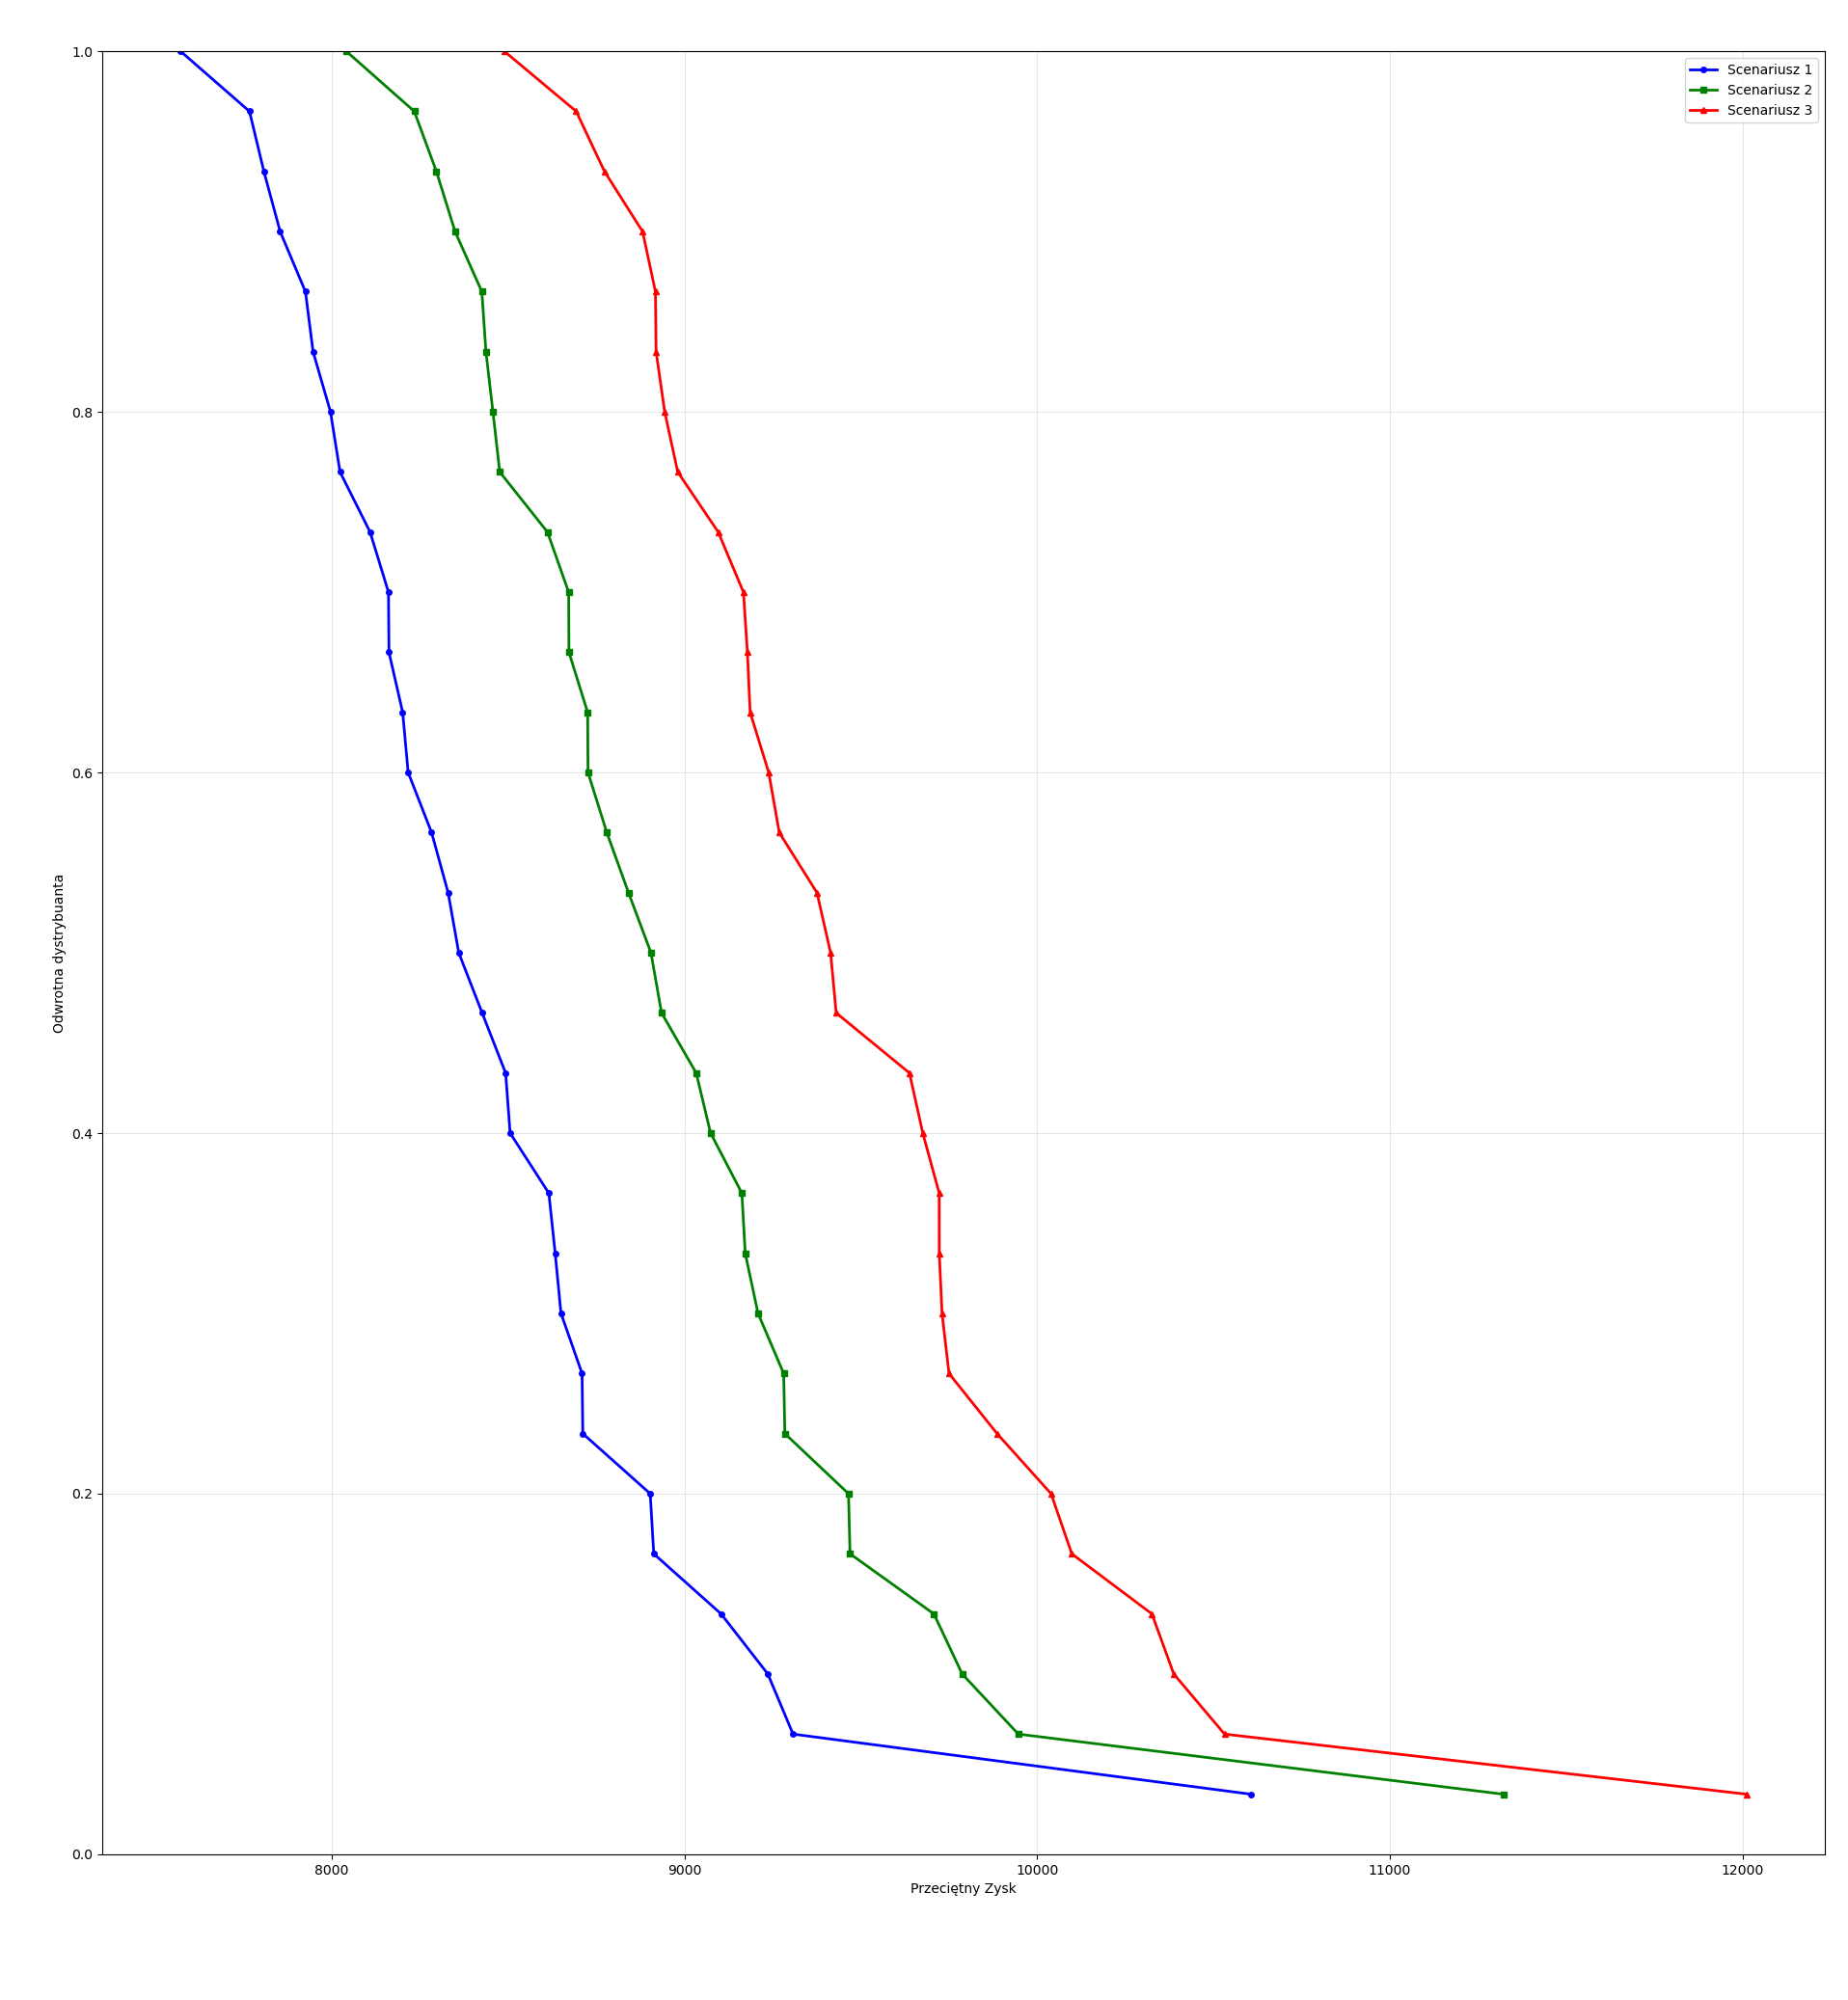
\includegraphics[width=\textwidth]{graphics/zysk_dystrybuanta.png}
\caption{Odwrotna dystrybuanta rozkładu średniego zysku między scenariuszami}
\label{fig:FSD-profit}
\end{figure}

Rysunek \ref{fig:FSD-risk} przedstawia odwrotną dystrybuantę rozkładu średniej różnicy Giniego jako miary ryzyka między scenariuszami dla tych samych trzech rozwiązań efektywnych. W kontekście miary ryzyka rozwiązanie A wykazuje dominację nad rozwiązaniami B i C, podczas gdy rozwiązanie B nie dominuje w sposób kategoryczny rozwiązania C. Przyczyna tego zjawiska jest związana z przecięciem się dystrybuant w punkcie oznaczonym kolorem żółtym na wykresie przedstawionym na rysunku \ref{fig:FSD-profit}.

\begin{figure}[ht!]
\centering
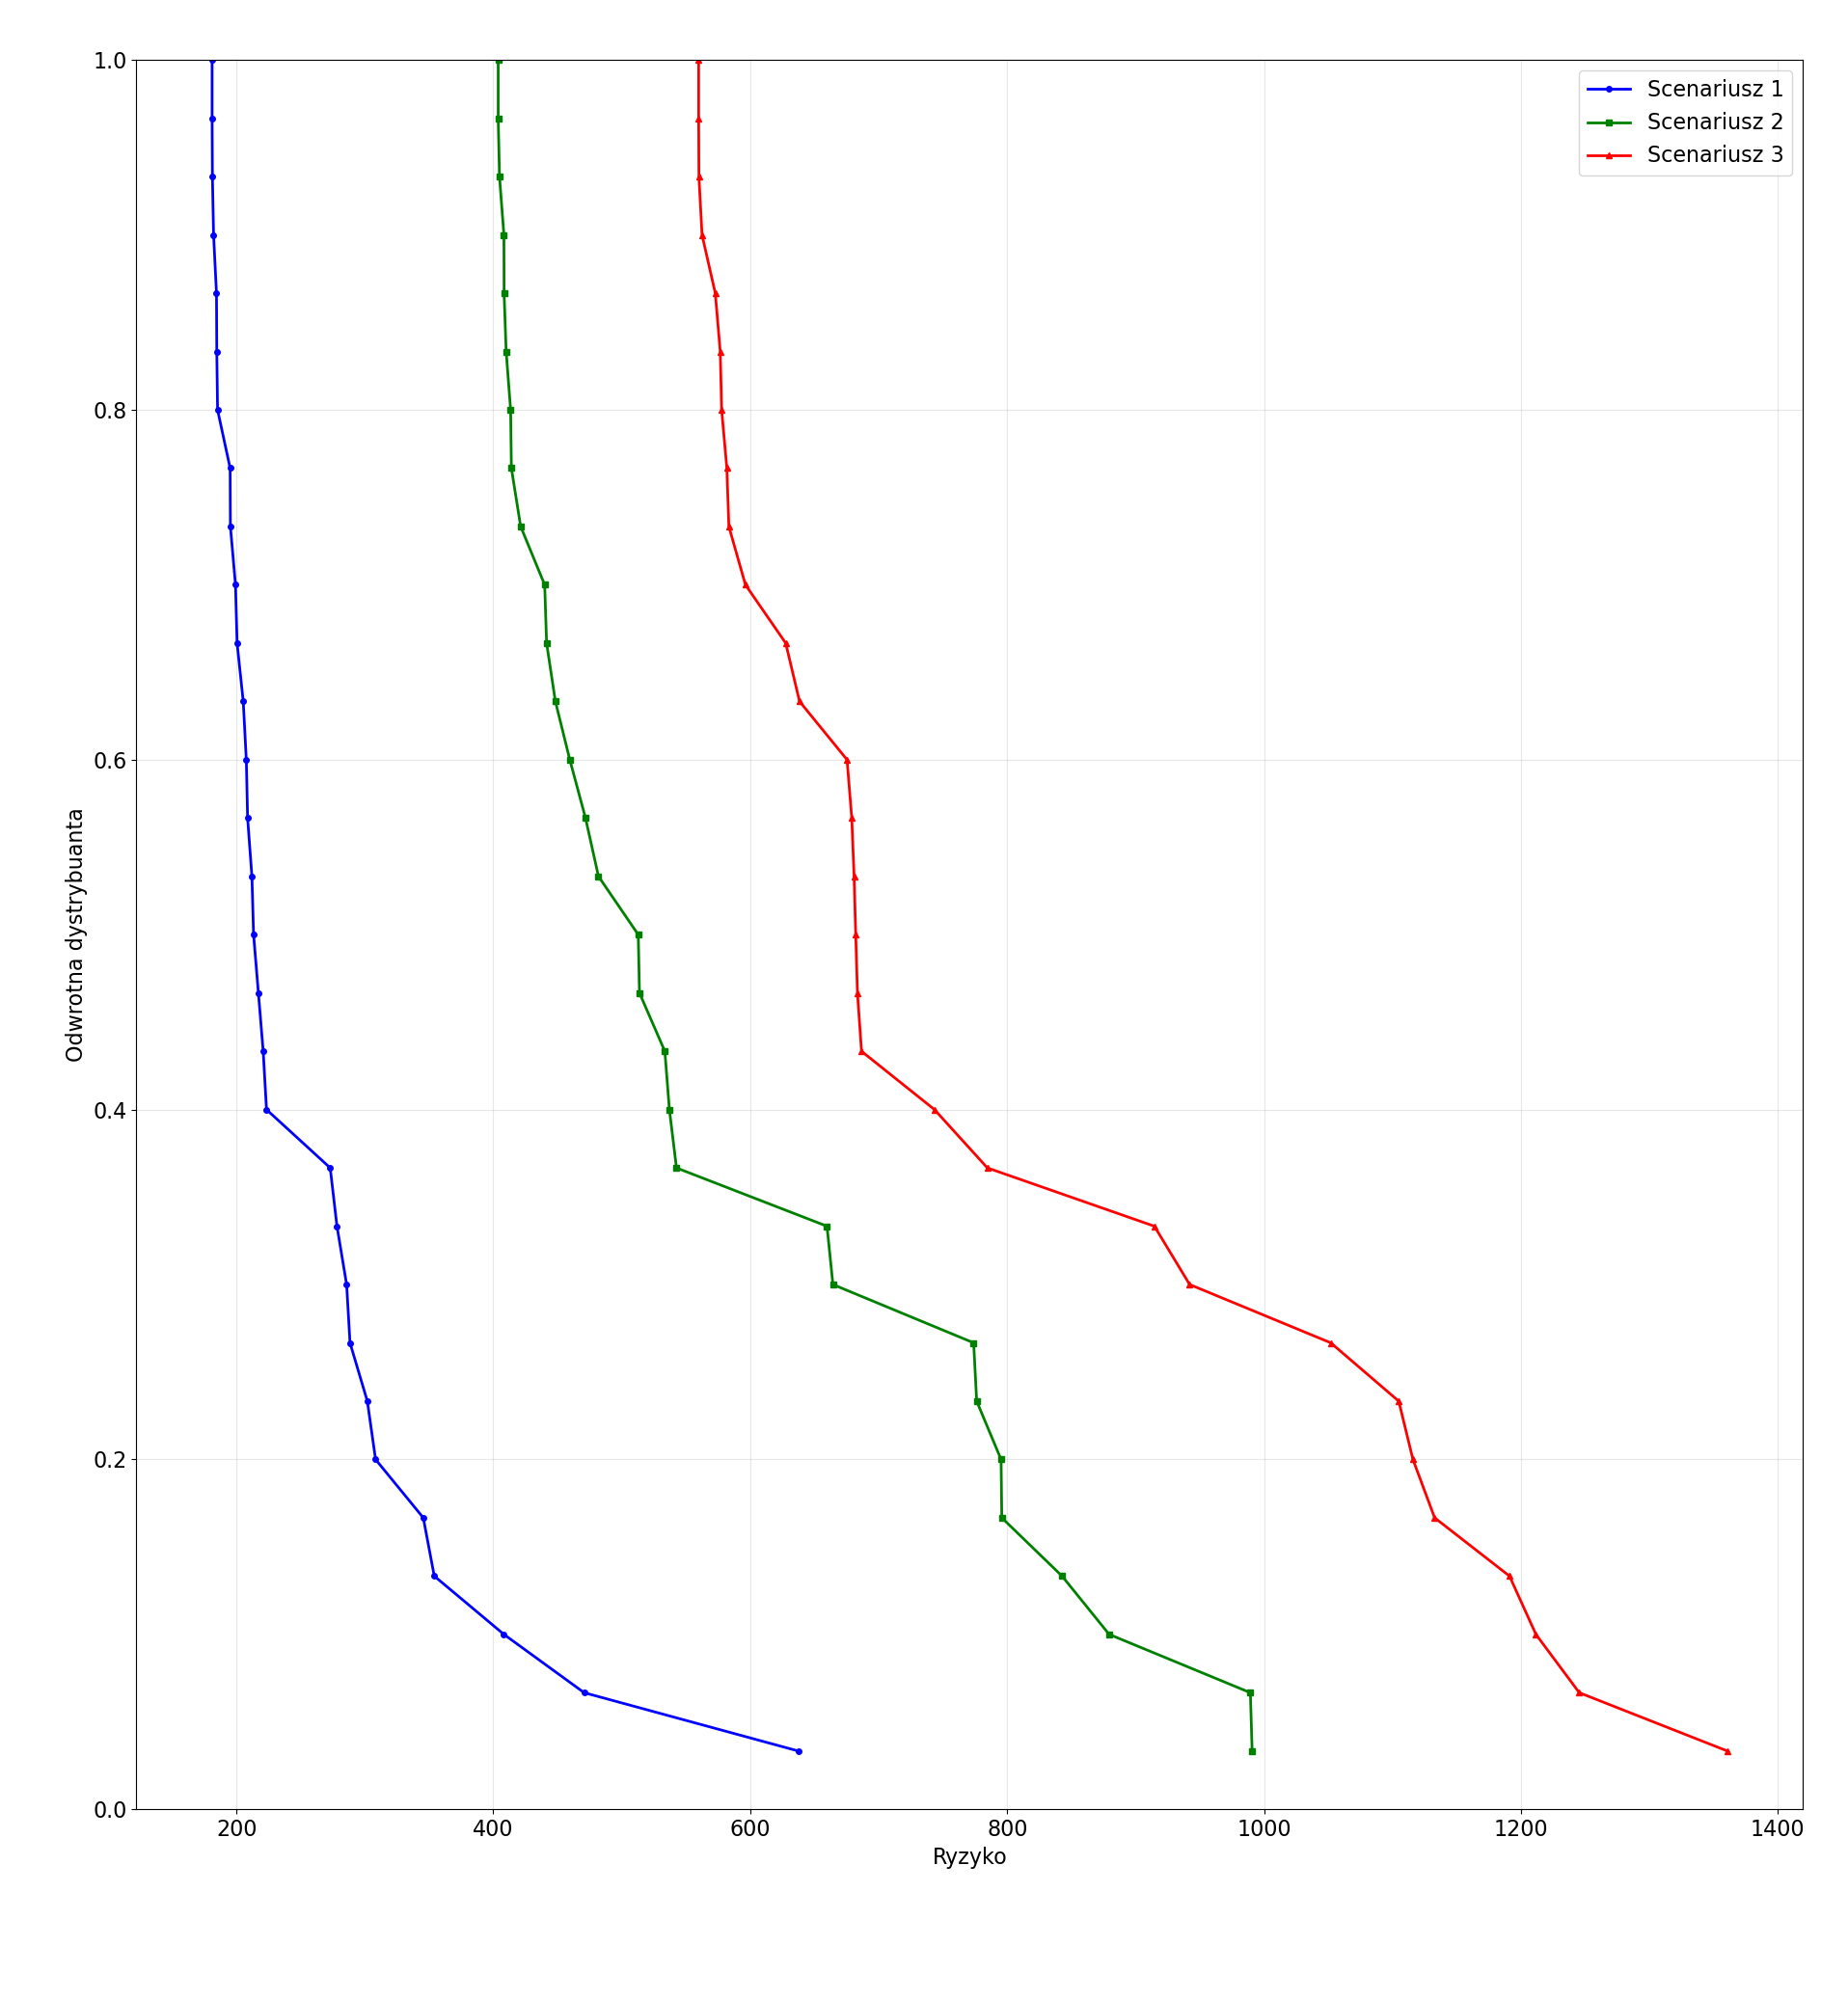
\includegraphics[width=\textwidth]{graphics/ryzyko_dystrybuanta.png}
\caption{Odwrotna dystrybuanta rozkładu średniej różnicy Giniego między scenariuszami}
\label{fig:FSD-risk}
\end{figure}


\end{document}